\documentclass{article}

\usepackage{fancyhdr}
\usepackage{extramarks}
\usepackage{amsmath}
\usepackage{amsthm}
\usepackage{amsfonts}
\usepackage{tikz}
\usepackage[plain]{algorithm}
\usepackage{algpseudocode}
\usepackage{subcaption}
\usepackage{authblk}
% \usepackage{subfigure}

\usetikzlibrary{automata,positioning}

%
% Basic Document Settings
%

\topmargin=-0.45in
\evensidemargin=0in
\oddsidemargin=0in
\textwidth=6.5in
\textheight=9.0in
\headsep=0.25in

\linespread{1.1}

\pagestyle{fancy}
\lhead{\hmwkAuthorName}
\chead{\hmwkClass\ (\hmwkClassInstructor\ \hmwkClassTime): \hmwkTitle}
\rhead{\firstxmark}
\lfoot{\lastxmark}
\cfoot{\thepage}

\renewcommand\headrulewidth{0.4pt}
\renewcommand\footrulewidth{0.4pt}

\setlength\parindent{0pt}

%
% Create Problem Sections
%

\newcommand{\enterProblemHeader}[1]{
    \nobreak\extramarks{}{Problem \arabic{#1} continued on next page\ldots}\nobreak{}
    \nobreak\extramarks{Problem \arabic{#1} (continued)}{Problem \arabic{#1} continued on next page\ldots}\nobreak{}
}

\newcommand{\exitProblemHeader}[1]{
    \nobreak\extramarks{Problem \arabic{#1} (continued)}{Problem \arabic{#1} continued on next page\ldots}\nobreak{}
    \stepcounter{#1}
    \nobreak\extramarks{Problem \arabic{#1}}{}\nobreak{}
}

\setcounter{secnumdepth}{0}
\newcounter{partCounter}
\newcounter{homeworkProblemCounter}
\setcounter{homeworkProblemCounter}{1}
\nobreak\extramarks{Problem \arabic{homeworkProblemCounter}}{}\nobreak{}

%
% Homework Problem Environment
%
% This environment takes an optional argument. When given, it will adjust the
% problem counter. This is useful for when the problems given for your
% assignment aren't sequential. See the last 3 problems of this template for an
% example.
%
\newenvironment{homeworkProblem}[1][-1]{
    \ifnum#1>0
        \setcounter{homeworkProblemCounter}{#1}
    \fi
    \section{Problem \arabic{homeworkProblemCounter}}
    \setcounter{partCounter}{1}
    \enterProblemHeader{homeworkProblemCounter}
}{
    \exitProblemHeader{homeworkProblemCounter}
}

%
% Homework Details
%   - Title
%   - Due date
%   - Class
%   - Section/Time
%   - Instructor
%   - Author
%

\newcommand{\hmwkTitle}{Assignment\ \#1}
\newcommand{\hmwkDueDate}{}
\newcommand{\hmwkClass}{EE2101 - Control Systems}
\newcommand{\hmwkClassTime}{}
\newcommand{\hmwkClassInstructor}{}
\newcommand{\hmwkAuthorName}{\textbf{Nikhil P}}
\newcommand{\hwkAuthorRollNo}{\textbf{EE19BTECH11026}}

%
% Title Page
%

\title{
    \vspace{2in}
    \textmd{\textbf{\hmwkClass\ \hmwkTitle}}\\
    % \normalsize\vspace{0.1in}\small{Due\ on\ \hmwkDueDate}\\
    \vspace{0.1in}\large{\textit{\hmwkClassInstructor\ \hmwkClassTime}}
    \vspace{3in}
}

\author{\hmwkAuthorName}
\affil{\hwkAuthorRollNo}
\date{}

\renewcommand{\part}[1]{\textbf{\large Part \Alph{partCounter}}\stepcounter{partCounter}\\}

%
% Various Helper Commands
%

% Useful for algorithms
\newcommand{\alg}[1]{\textsc{\bfseries \footnotesize #1}}

% For derivatives
\newcommand{\deriv}[1]{\frac{\mathrm{d}}{\mathrm{d}x} (#1)}

% For partial derivatives
\newcommand{\pderiv}[2]{\frac{\partial}{\partial #1} (#2)}

% Integral dx
\newcommand{\dx}{\mathrm{d}x}

% Alias for the Solution section header
\newcommand{\solution}{\textbf{\large Solution}}

% Probability commands: Expectation, Variance, Covariance, Bias
\newcommand{\E}{\mathrm{E}}
\newcommand{\Var}{\mathrm{Var}}
\newcommand{\Cov}{\mathrm{Cov}}
\newcommand{\Bias}{\mathrm{Bias}}

\begin{document}

\maketitle

\pagebreak

\begin{homeworkProblem}
    \textbf{Q28)}Find the Transfer function $\frac{X_3(s)}{F(s)}$ for each of the following:
    
    \textbf{Part One}
    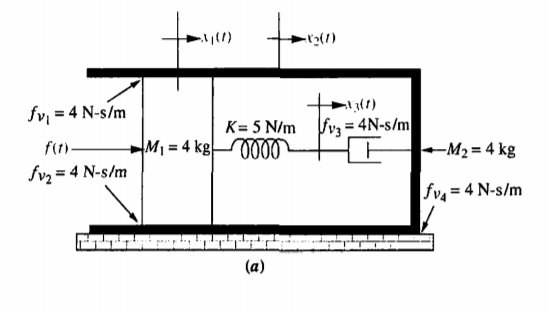
\includegraphics[width=0.6\linewidth]{figures/q1a.png}
    
    \textbf{Solution}
    Since there are three degrees of freedom, there must be 3 equations of motion
    Considering only $M_1$,
% \begin{figure}[h]

% \begin{subfigure}{0.5\textwidth}
% 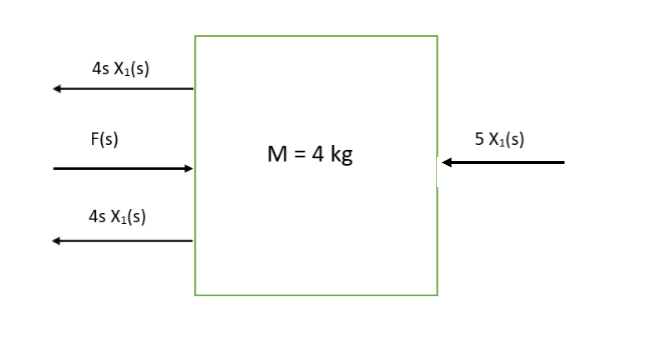
\includegraphics[width=0.9\linewidth, height=5cm]{figures/a1m1x1.png} 
% \caption{Forces due to displacement $x_1(t)$}
% % \label{fig:a1m1x1}
% \end{subfigure}
% \begin{subfigure}{0.5\textwidth}
% 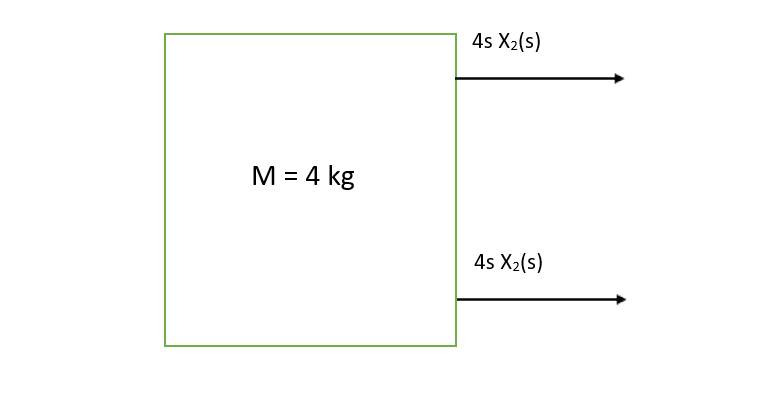
\includegraphics[width=0.9\linewidth, height=5cm]{figures/a1m1x2.png}
% \caption{ Forces due to displacement $x_2(t)$}
% % \label{fig:a1m1x2}
% \end{subfigure}

% \caption{Caption for this figure with two images}
% % \label{fig:image2}

% \end{figure}

\begin{figure}[H]
\centering
\subcaptionbox{Forces due to displacement $x_1(t)$}{%
  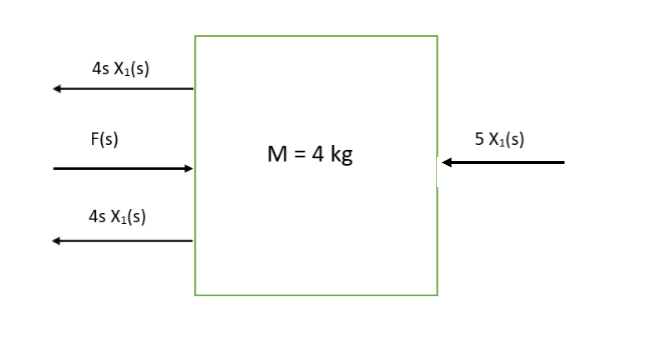
\includegraphics[width=0.45\textwidth]{figures/a1m1x1.png}}\hfill
\subcaptionbox{Forces due to displacement $x_2(t)$}{%
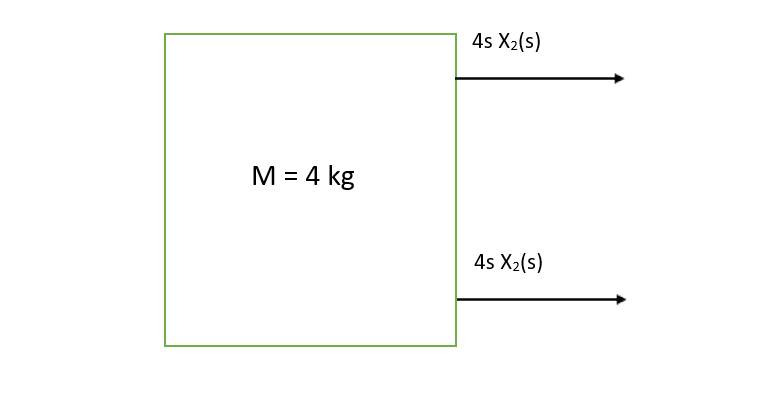
\includegraphics[width=0.45\textwidth]{figures/a1m1x2.png}}\par
\subcaptionbox{Forces due to displacement $x_3(t)$}{%
  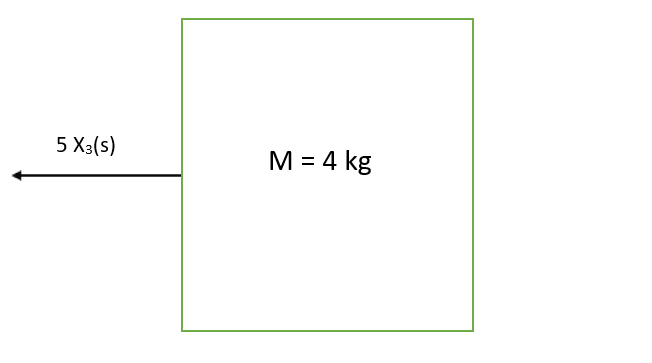
\includegraphics[width=0.45\textwidth]{figures/a1m1x3.png}} \hfill
\subcaptionbox{Total Forces}{%
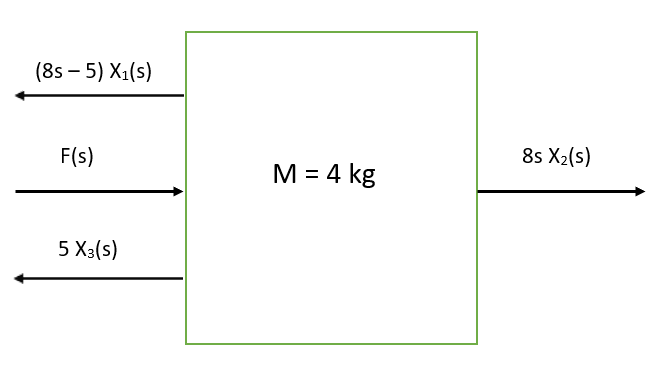
\includegraphics[width=0.45\textwidth]{figures/a1m1all.png}}\par
\end{figure}

We get the equation:
\begin{equation}
    \centering
    F(s) = (4 s^2 + 8s + 5)X_1(s) - 8s X_2(s) - 5 X_3(s)
\label{a1m1}
\end{equation}

Similarly, doing this with $M_2$,

\begin{figure}[H]
\centering
\subcaptionbox{Forces due to displacement $x_1(t)$}{%
  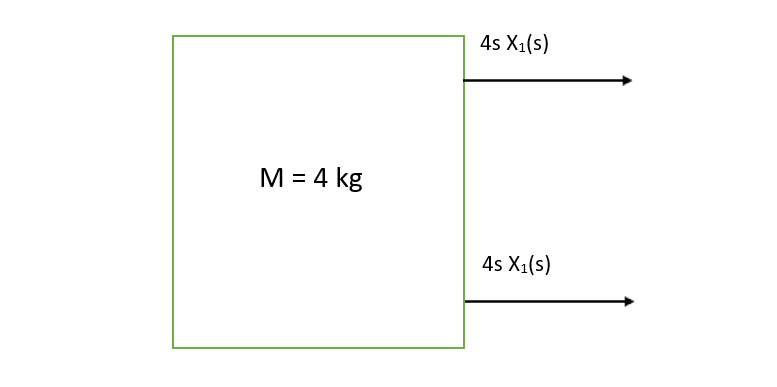
\includegraphics[width=0.45\textwidth]{figures/a1m2x1.png}}\hfill
\subcaptionbox{Forces due to displacement $x_2(t)$}{%
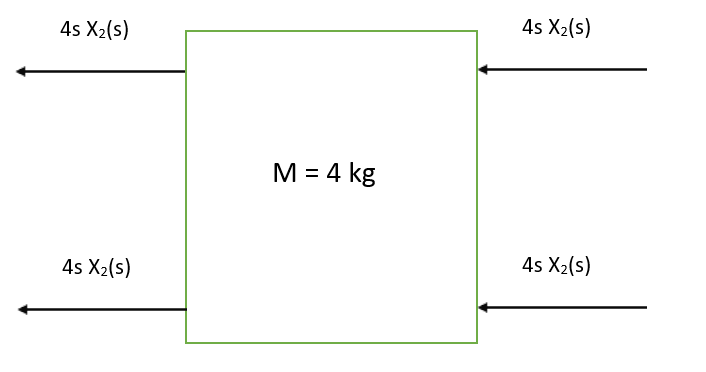
\includegraphics[width=0.45\textwidth]{figures/a1m2x2.png}}\par
\subcaptionbox{Forces due to displacement $x_3(t)$}{%
  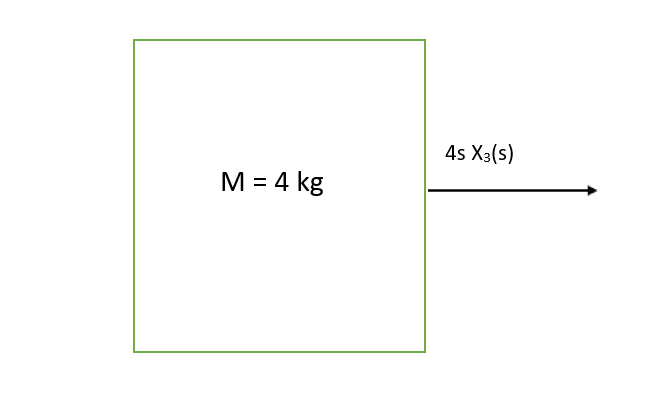
\includegraphics[width=0.45\textwidth]{figures/a1m2x3.png}} \hfill
\subcaptionbox{Total Forces}{%
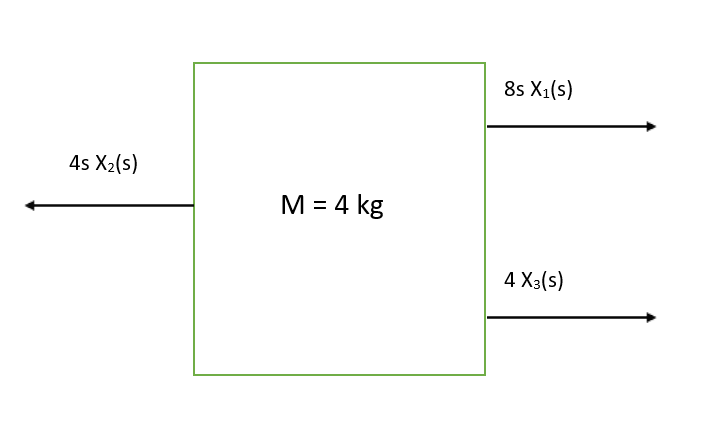
\includegraphics[width=0.45\textwidth]{figures/a1m2all.png}}\par
\end{figure}

\begin{equation}
    \centering
    8sX_1(s) -(4s^2 + 16s)X_2(s) + 4s X_3(s) = 0
\label{a1m2}
\end{equation}

Now, for the 3rd equation, we consider the point of contact of the damper and spring. Since the mass of the point is 0, the sum of all forces at that point must be zero

\begin{equation}
    \centering
    5 X_1(s) + 4sX_2(s) - (4s+ 5) X_3(s) = 0
\label{a1m2}
\end{equation}

Constructing a Matrix, we get
\begin{equation*}
\centering
\begin{bmatrix}
    4 s^2 + 8s + 5 & - 8s & - 5 \\
    8s & -4s - 16s & 4s \\
    5 & + 4s & - 4s- 5
\end{bmatrix}   \begin{bmatrix}
    X_1(s) \\
    X_2(s) \\
    X_3(s)
\end{bmatrix} = 
\begin{bmatrix}
    F(s) \\
    0 \\
    0
\end{bmatrix} \\
\centering
\implies X_3 = \frac{\Delta_3}{\Delta} \\
\centering
\text{,where} \Delta = \begin{vmatrix}
    4 s^2 + 8s + 5 & - 8s & - 5 \\
    8s & -4s - 16s & 4s \\
    5 & + 4s & - 4s- 5
\end{vmatrix} \\

\centering
\Delta_3 = \begin{vmatrix}
    4 s^2 + 8s + 5 & - 8s & F(s) \\
    8s & -4s - 16s & 0 \\
    5 & + 4s & 0
\end{vmatrix} \\

\end{equation*}

Solving, we get
\begin{align}
    X_3(s) = \frac{F(s)(13 s + 20)}{16 s^4 + 100 s^3 + 172 s^2 + 60 s} \\
    \implies \frac{X_3(s)}{F(s)} = \frac{(13 s + 20)}{16 s^4 + 100 s^3 + 172 s^2 + 60 s}
\end{align}




\textbf{Part Two}

    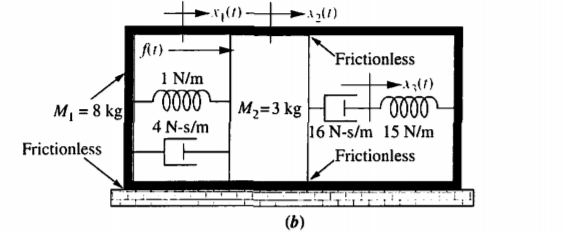
\includegraphics[width=0.6\linewidth]{figures/q1b.png}
    
    \textbf{Solution}
    Since there are three degrees of freedom, there must be 3 equations of motion
    Considering only $M_1$,



\begin{figure}[H]
\centering
\subcaptionbox{Forces due to displacement $x_1(t)$}{%
  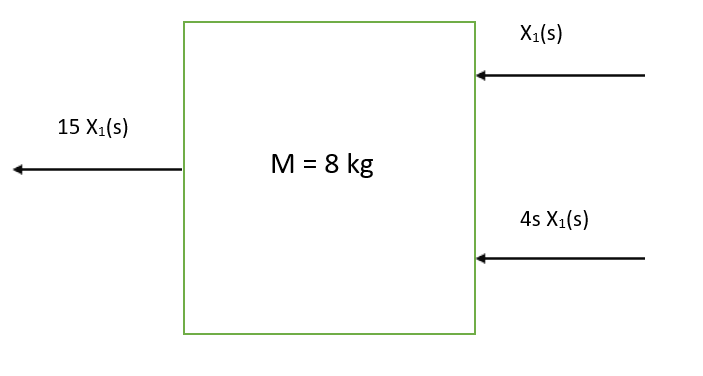
\includegraphics[width=0.45\textwidth]{figures/a2m1x1.png}}\hfill
\subcaptionbox{Forces due to displacement $x_2(t)$}{%
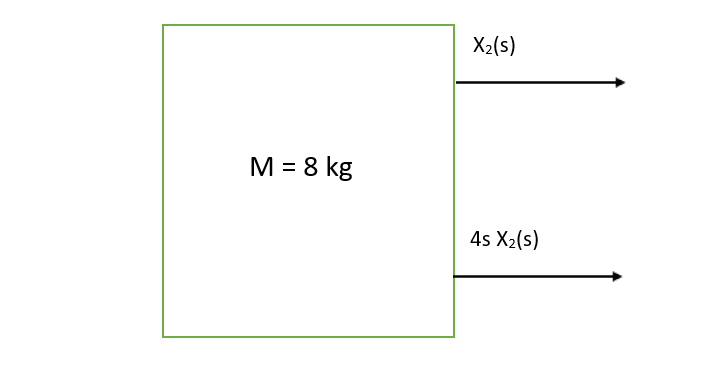
\includegraphics[width=0.45\textwidth]{figures/a2m1x2.png}}\par
\subcaptionbox{Forces due to displacement $x_3(t)$}{%
  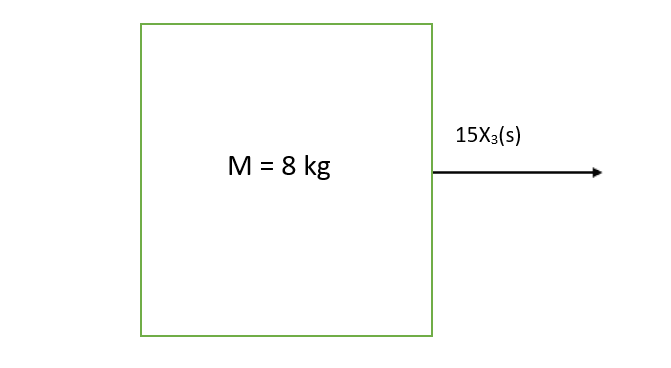
\includegraphics[width=0.45\textwidth]{figures/a2m1x3.png}} \hfill
\subcaptionbox{Total Forces}{%
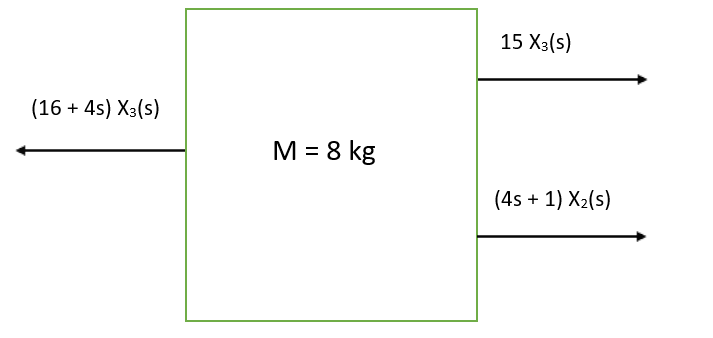
\includegraphics[width=0.45\textwidth]{figures/a2m1all.png}}\par
\end{figure}

We get the equation:
\begin{equation}
    \centering
    (8 s^2 + 4s + 16)X_1(s) - (4s + 1) X_2(s) - 15 X_3(s) = 0
\label{a1m1}
\end{equation}

Similarly, doing this with $M_2$,

\begin{figure}[H]
\centering
\subcaptionbox{Forces due to displacement $x_1(t)$}{%
  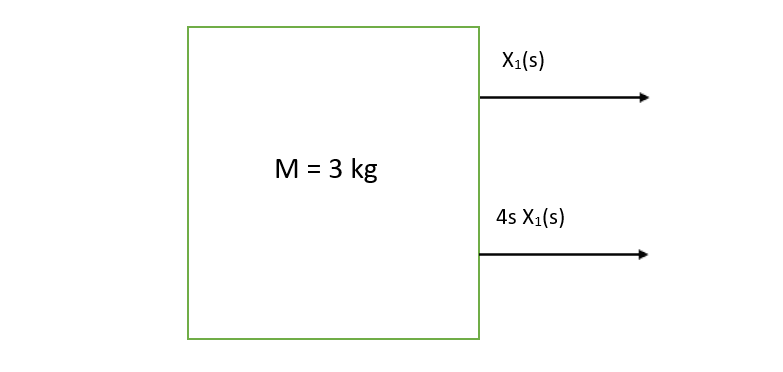
\includegraphics[width=0.45\textwidth]{figures/a2m2x1.png}}\hfill
\subcaptionbox{Forces due to displacement $x_2(t)$}{%
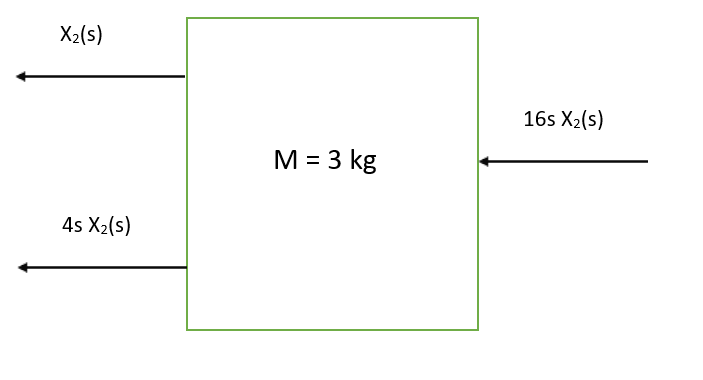
\includegraphics[width=0.45\textwidth]{figures/a2m2x2.png}}\par
\subcaptionbox{Forces due to displacement $x_3(t)$}{%
  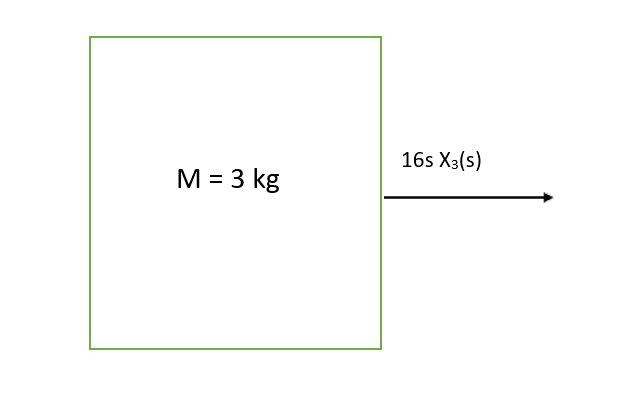
\includegraphics[width=0.45\textwidth]{figures/a2m2x3.png}} \hfill
\subcaptionbox{Total Forces}{%
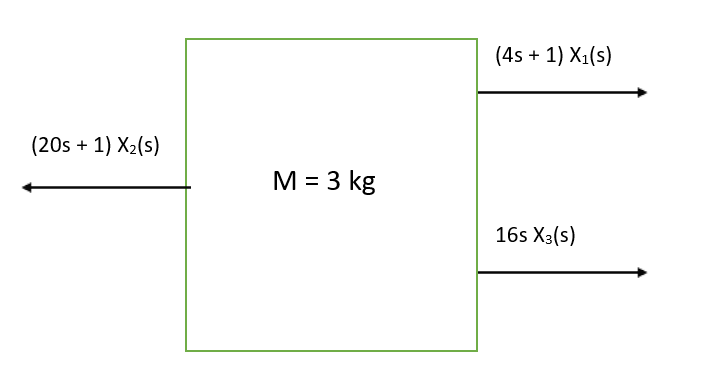
\includegraphics[width=0.45\textwidth]{figures/a2m2all.png}}\par
\end{figure}

\begin{equation}
    \centering
    -(4s + 1)X_1(s) +(3s^2 + 20s + 1)X_2(s) + 16s X_3(s) = F(s)
\label{a1m2}
\end{equation}

Now, for the 3rd equation, we consider the point of contact of the damper and spring. Since the mass of the point is 0, the sum of all forces at that point must be zero

\begin{equation}
    \centering
    15 X_1(s) + 16sX_2(s) - (16s+ 15) X_3(s) = 0
\label{a1m2}
\end{equation}

Constructing a Matrix, we get
\begin{equation*}
\centering
\begin{bmatrix}
    8 s^2 + 4s + 16 & - (4s + 1) & - 15  \\
     -(4s + 1) & +(3s^2 + 20s + 1) &  16s\\
    15 & 16s & - (16s+ 15) 
\end{bmatrix}   \begin{bmatrix}
    X_1(s) \\
    X_2(s) \\
    X_3(s)
\end{bmatrix} = 
\begin{bmatrix}
    0 \\
    F(s) \\
    0
\end{bmatrix} \\
\centering
\implies X_3 = \frac{\Delta_3}{\Delta} \\
\centering
\text{,where} \Delta = \begin{vmatrix}
    8 s^2 + 4s + 16 & - (4s + 1) & - 15  \\
     -(4s + 1) & +(3s^2 + 20s + 1) &  16s\\
    15 & 16s & - (16s+ 15) 
\end{vmatrix}  \\

\centering
\Delta_3 = \begin{vmatrix}
    8 s^2 + 4s + 16 & - (4s + 1) & 0  \\
     -(4s + 1) & +(3s^2 + 20s + 1) &  F(s)\\
    15 & 16s &  0
\end{vmatrix} \\

\end{equation*}

Solving, we get
\begin{align}
    X_3(s) = \frac{F(s)(128s^3 + 64 s^2 + 316 s + 15)}{384 s^5 + 1064 s^4 + 3476 s^3 + 165 s^2} \\
    \implies \frac{X_3(s)}{F(s)} = \frac{(128s^3 + 64 s^2 + 316 s + 15)}{384 s^5 + 1064 s^4 + 3476 s^3 + 165 s^2} 
\end{align}


\end{homeworkProblem}


\end{document}
